\section{Pruebas}
\label{sec:pruebas}
\subsection{Introducción}
\noindent Para contrastar el funcionamiento de las tareas realizadas conforme a los objetivos fijados, se van a realizar una serie de pruebas para cada tipo de clasificación. \\

\section *{Métricas}
\noindent A continuación se exponen los experimentos realizados, así como la característica medida.

\begin{itemize}
	\item Medidas de rendimiento.
		\begin{itemize}
			\item Precisión frente a velocidad en clasificación dinámica.
			\item Precisión frente a exhaustividad en clasificación estática con misma configuración de objetos.
			\item Obtención del valor F para los valores de precisión y exhaustividad nombrados en el punto anterior.
			\item Precisión en robótica adaptativa.
		\end{itemize}
	\item Medidas de error. Estas se realizan tanto en entorno estático como dinámico.
		\begin{itemize}
			\item Precisión frente a número de objetos.
			\item Precisión frente a tamaño de objetos.
		\end{itemize}
\end{itemize}

	%\item Tiempo que tarda la clasificación estática frente a la dinámica.
	


\section*{Resultados}
\subsection{Medidas de rendimiento}
\noindent A continuación se muestran los resultados obtenidos para las pruebas de rendimiento. \\
\subsubsection{Precisión frente a velocidad en clasificación dinámica}
\noindent Para esta prueba, se han realizado unas 25 ejecuciones con distintas configuraciones (posición que toma cada objeto). Como vemos en la gráfica \ref{cd:ve}, cuanto mayor es la velocidad, menor es la precisión que se obtiene.\\

\begin{figure}[H]
	\centering % si queremos la imagen centrada
	\label{cd:ve}
	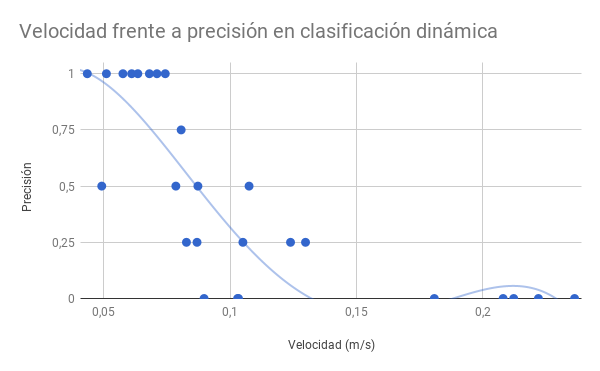
\includegraphics[scale=0.55]{imagenes/vel-eficiencia.png}
	\caption{Gráfica que muestra la velocidad frente a la eficiencia en clasificación dinámica con cuña donde la línea sigue un ajuste polinómico de grado 6.}
\end{figure}

%\begin{figure}[H]
%	\centering % si queremos la imagen centrada
%	\label{cd:areave}
%	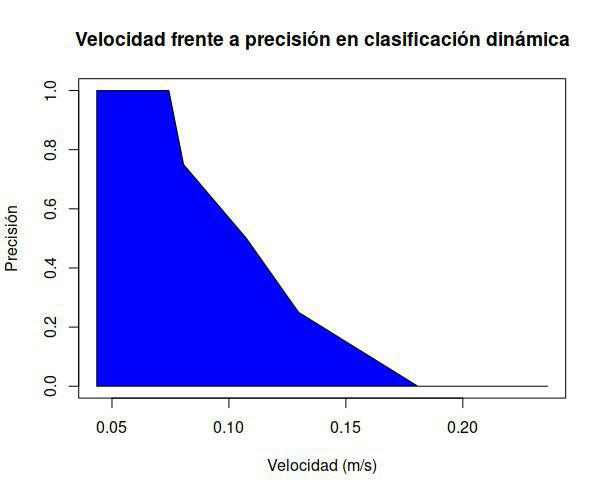
\includegraphics[scale=0.55]{imagenes/areave.jpg}
%	\caption{Gráfica que muestra la curva seguida por la velocidad frente a la precisión en clasificación dinámica con cuña}
%\end{figure}

\noindent Se ha realizado un ajuste de los datos obtenidos con una línea de tendencia de tipo polinómica de grado 4 y se ha obtenido la figura anterior \ref{cd:ve}. Los resultados obtenidos siguen una curva lógica, siendo los valores de precisión más bajos cuanta más velocidad lleva la cinta transportadora. Es por esto por lo que las siguientes pruebas que se realicen en un entorno dinámico se ejecutarán con una velocidad menor a 0.1 m/s. Sin embargo, si nos fijamos en la gráfica \ref{cd:ve}, podemos observar algunos puntos algo dispares con respecto a la media; esto puede deberse al algoritmo de planificación de MoveIt! utilizado, como se explicaba en la sección \ref{planif}. \\

\subsubsection{Precisión y exhaustividad}
\noindent Estos valores, utilizados en medicina como especificidad, \textit{``specificity''} y sensitividad, \textit{``sensitivity''} \cite{powers2011evaluation}, también pueden ser de ayuda a la hora de comparar un algoritmo de clasificación con otro. Para explicarlos, se va a mostrar un ejemplo tras definir estos conceptos.  \cite{pr} \\

\noindent A la hora de realizar una clasificación, se denomina al trabajo realizado de 4 posibles maneras fijándonos en el número de objetos verdes: \\

\begin{itemize}
	\item \textbf{Verdadero positivo}. En esta prueba, son aquellos objetos verdes que Baxter ha separado y que realmente eran verdes.
	\item \textbf{Verdadero negativo}. Son los objetos separados como verdes, pero que realmente son azules.
	\item \textbf{Falso positivo}. Son aquellos objetos azules que no se han separado.
	\item \textbf{Falso negativo}. Son los objetos verdes que han quedado por separar. \\
\end{itemize}

\noindent El valor de precisión, ``precision'', se refiere a los objetos clasificados como positivos que realmente son verdaderos positivos, mientras que la exhaustividad o ``recall'' es el ratio de verdaderos positivos. \\
\noindent Así, si tenemos un conjunto de 4 objetos verdes y 4 azules \ref{cd:clasif} y separamos 2 verdes y 1 azul, la precisión será 2/3 y la exhaustividad 2/4. Es decir, habremos separado únicamente 2 objetos que realmente son verdes de 4 objetos verdes que había en total. \\

\begin{figure}[H]
	\centering
	\label{cd:clasif}
	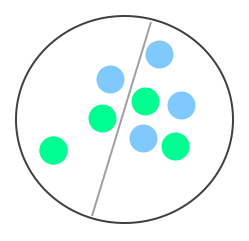
\includegraphics[scale=0.55]{imagenes/clasif.png}
	\caption{Ejemplo de precisión y exhaustividad en el que se ven los objetos que toma como verdaderos positivos (a la izquierda) y los que toma como negativos (a la derecha).}
\end{figure}

\noindent Para esta prueba, se ha realizado una modificación en el programa de clasificación estática, de forma que se pueda cambiar un parámetro ``\textit{precision}'' que permita separar en mayor o menor porcentaje el número de objetos de un color, de manera que se pueda medir la precisión y exhaustividad que se obtienen para unos valores predefinidos. \\

\noindent Se han realizado ejecuciones para valores del parámetro ``\textit{precision}'' de 0.5, 0.7 y 0.9 con 3 objetos de cada color, verde y azul. A continuación se muestra la gráfica de curvas PR, que consiste en una compensación entre precisión y exhaustividad para un diferente umbral, en este caso, el parámetro ``\textit{precision}''.\\

\begin{figure}[H]
	\centering
	\label{cd:pr}
	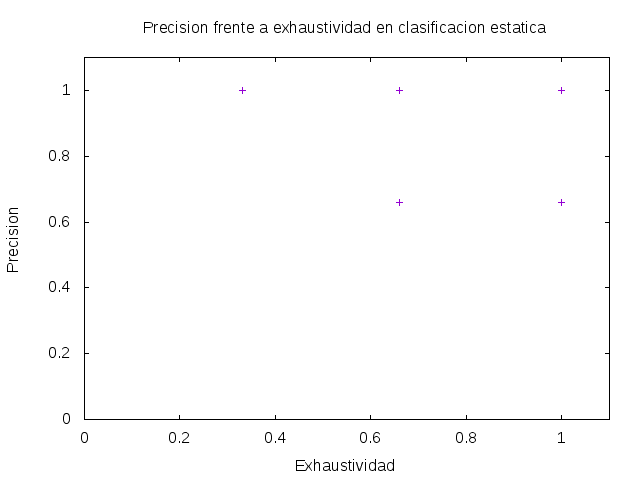
\includegraphics[scale=0.55]{imagenes/PR2.png}
	\caption{Gráfica que muestra la exhaustividad frente a la precisión en clasificación estática}
\end{figure}

%\noindent Para realizar el ajuste, se ha utilizado una línea de tendencia polinómica de grado 6. En este caso, los datos no son lo suficientemente significativos como para realizar esta curva, no existe ninguna función que siga los puntos obtenidos, esta es la mejor aproximación que se puede obtener. \\
\noindent El número de objetos de los que se dispone es de 3 de cada color, por lo que los valores de precisión y exhaustividad únicamente son 0.33, 0.66 y 0.99, ya que se obtienen en función del número de objetos verdes separados. No se ha realizado ninguna curva de ajuste ya que con los únicos datos que se pueden obtener no existe ninguna función que pueda aproximarse a ellos. \\

\noindent La alta precisión observada en la gráfica indica un bajo ratio de falsos positivos, mientras que un valor alto de exhaustividad indica un bajo ratio de falsos negativos \cite{scikit-learn}. En nuestro caso, la gráfica presenta valores altos para precisión y exhaustividad, por lo que se puede decir que los resultados son positivos, obteniendo una alta eficacia para los objetos clasificados. \\

\noindent Otra medida recurrente en este tipo de curvas consiste en calcular el valor F \cite{powers2011evaluation}, equivalente a la media armónica. Este valor une las dos medidas, precisión y exhaustividad, cuando sus valores son cercanos, de forma que podamos realizar comparativas de algoritmos con una sola variable. Su fórmula cuando la importancia que se le da a ambas medidas es la misma, es la siguiente: \\

%\centering
$ F_{1} = 2 * (precision * exhaustividad)/(precision + exhaustividad) $ \\

\noindent En caso de que no se le dé el mismo peso a ambas medidas se utiliza la siguiente fórmula: \\

$ F_{\beta} = (1 + \beta^{2}) * (precision/exhaustividad) / (\beta^{2} * precision + exhaustividad)$ \\

\noindent Ya que es una medida ponderada, en esta prueba se utilizará F2, una variante en la que se da más peso a la exhaustividad frente a la precisión, es decir, en nuestro caso, se intenta que se separe el mayor número de objetos verdes, aunque además se clasifique alguno azul con estos. La fórmula para ello es la siguiente: \\

$ F_{2} = 5 * (precision * exhaustividad)/(4* precision + exhaustividad) $ \\

\noindent Calculándolo para cada uno de los valores obtenidos en precisión y exhaustividad y quedándonos con el valor más alto se obtiene: $ F2 = 1 $, seguido de $ F2 = 0.9066 $.\\ 

\noindent Puesto que este valor es la media de ambas medidas precisión y exhaustividad, podemos decir que, como se explicó anteriormente, las pruebas realizadas para este número de objetos presentan una alta eficacia, separándose el mayor número de verdes posible. \\

\subsubsection{Robótica adaptativa}
\noindent Para esta implementación, se ha utilizado el código de clasificación en entorno estático. A partir de este, se ha definido una variable booleana que indica cuándo la segmentación se debe enfocar de forma adaptativa. Cuando esta variable se establece como \textit{True}, el programa preguntará la precisión obtenida en la ejecución anterior en un rango de [0:1] y la guardará en una variable. Como caso inicial, esta se debe establecer a -1. \\

\noindent A partir de este parámetro modificado a través de línea de comandos que llamaremos \textit{``precision\_value''} y otro valor \textit{alpha} inicializado a 0.1, el programa se encarga de alterar el valor de la coordenada \textit{x}, que en el caso de Baxter corresponde a la coordenada en el eje de ordenadas. De esta forma, cuanto menor sea el valor de \textit{``precision\_value''}, mayor será la modificación de la coordenada \textit{x}, que hará que el brazo de Baxter se sitúe más arriba, alcanzando más objetos de un mismo color. \\

\noindent Para mostrar el funcionamiento de esta aproximación se expone una tabla a partir de algunos resultados obtenidos, que consta del valor de precisión ``\textit{precision\_value}'' que se le proporciona en cada ejecución y de la precisión que realmente se obtiene. Se han utilizado 6 objetos, 3 de cada color, por lo que los valores de precisión que se pueden obtener son únicamente 0, 0.33, 0.66 y 1.

\begin{table}[H]
	\centering
	\begin{tabular}{|p{4cm} | p{4cm} |}
		\hline
		\textbf{\textit{precision\_value}} & \textbf{Precisión obtenida} \\ 
		\hline
		-1.0 & 1.0 \\
		\hline
		-1.0 & 0.66 \\
		\hline
		0.66 & 1.0 \\
		\hline
		0.66 & 0.66 \\
		\hline
		0.33 & 1.0 \\
		\hline
		0.0 & 1.0 \\
		\hline
		0.0 & 0.66 \\
		\hline
	\end{tabular}
	\caption{Tabla que muestra la precisión que se le indica al programa en cada ejecución y la precisión obtenida realmente.}
	\label{cuad:radap}
\end{table}

\noindent Al constar de pocos objetos, es difícil ver si realmente se ha mejorado la precisión. En la tabla se han incluido todas las combinaciones de resultados obtenidas en las 20 pruebas realizadas y, como se puede ver, cuanto menor es el valor que se le proporciona, mayor es la alteración de la coordenada \textit{x}, de manera que se mejore más eficazmente la precisión que se obtenga. \\

\subsection{Medidas de error}
\noindent Estas pruebas se han realizado tanto en clasificación dinámica como en estática. Es necesario tener en cuenta el tamaño de la cinta transportadora, ya que esta es bastante estrecha y no caben muchos objetos, de esta forma, se han realizado las ejecuciones para 4, 6 y 7 objetos de distinto tamaño.\\

\subsubsection{Clasificación estática}
\noindent Veremos primero los resultados obtenidos con objetos grandes y a continuación con objetos pequeños. \\
\begin{itemize}
	\item \textbf{Objetos grandes} \\
	\noindent En primer lugar, vemos la gráfica obtenida para configuraciones de objetos grandes de 4, 6 y 7 unidades. \\
	\begin{figure}[H]
		\centering % si queremos la imagen centrada
		\label{cd:eg}
		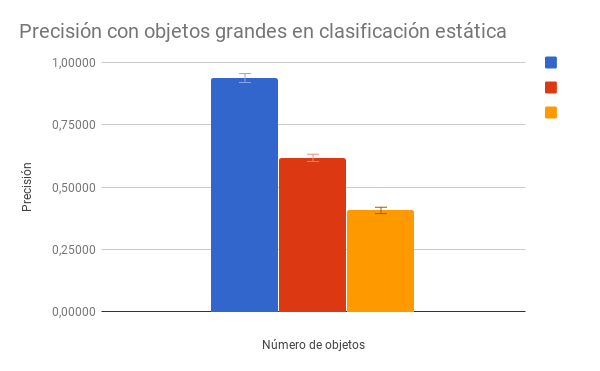
\includegraphics[scale=0.55]{imagenes/errbar_eg.png}
		\caption{Gráfica que muestra el número de objetos grandes frente a la precisión en clasificación estática, representando la media con una columna y la desviación típica con una barra.}
	\end{figure}

	\noindent En esta gráfica, se ha representado con un punto la media de los valores de precisión obtenidos en las ejecuciones para 4, 6 y 7 objetos, a la que se ha añadido una barra de error equivalente a la desviación estándar para el conjunto de resultados obtenidos con ese número de objetos. En este caso, no existe una gran variación de precisión en las ejecuciones, por lo que se ajusta bastante a la media. Como era de esperar, cuantos más objetos haya en la mesa, menos precisión se obtiene, puesto que la herramienta de la que se dispone no presenta la longitud adecuada para separar todos los objetos. \\
	
	\item \textbf{Objetos pequeños}
	\begin{figure}[H]
		\centering % si queremos la imagen centrada
		\label{cd:ep}
		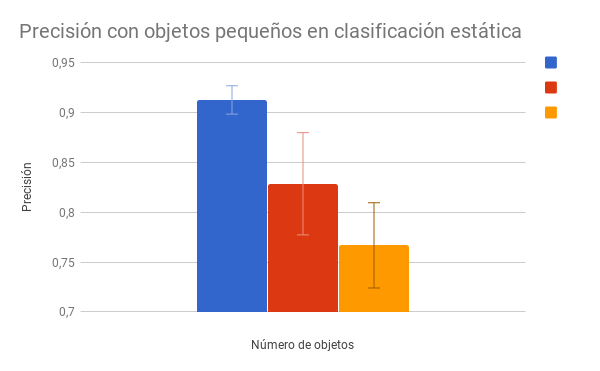
\includegraphics[scale=0.55]{imagenes/errbox_ep.png}
		\caption{Gráfica que muestra el número de objetos pequeños frente a la precisión en clasificación estática, representando la media con una columna y la desviación típica con una barra.}
	\end{figure}
	
	\noindent En este caso, vemos que la media de los valores obtenidos es bastante alta para las 3 configuraciones, ya que al ser más pequeños, la herramienta que en este caso lleva Baxter alcanza a la mayoría de ellos; si nos fijamos en la barra de error, para la configuración de 6 y de 7 objetos es más amplia, por lo que sabemos que ha habido más ejecuciones en las que no se han separado todos los objetos de un mismo color. \\
	
\end{itemize}

\subsubsection{Clasificación dinámica}
\noindent Del mismo modo que en la anterior, veremos primero los resultados con objetos grandes y después con pequeños, esta vez para clasificación en entorno dinámico utilizando una cuña como herramienta. \\

\begin{itemize}
	\item \textbf{Objetos grandes}

	\begin{figure}[H]
		\centering % si queremos la imagen centrada
		\label{cd:dg}
		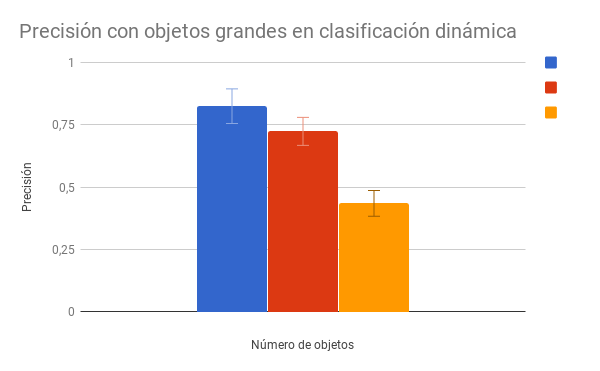
\includegraphics[scale=0.55]{imagenes/errbar_dg.png}
		\caption{Gráfica que muestra el número de objetos grandes frente a la precisión en clasificación dinámica con cuña, representando la media con una columna y la desviación típica con una barra.}
	\end{figure}

	\noindent Como muestra la figura, los resultados son bastante parecidos a los que nos encontramos en clasificación estática, aunque en este caso la barra de error o desviación estándar vuelve a ser más amplia. Esto se debe a que los objetos son grandes y de madera, Baxter sujeta la cuña de cartón con el \textit{gripper}, por lo que en algunas ocasiones el peso de los objetos vence la fuerza del \textit{gripper}, del que se resbala la cuña.\\

	\item \textbf{Objetos pequeños}
	
	\begin{figure}[H]
		\centering % si queremos la imagen centrada
		\label{cd:dp}
		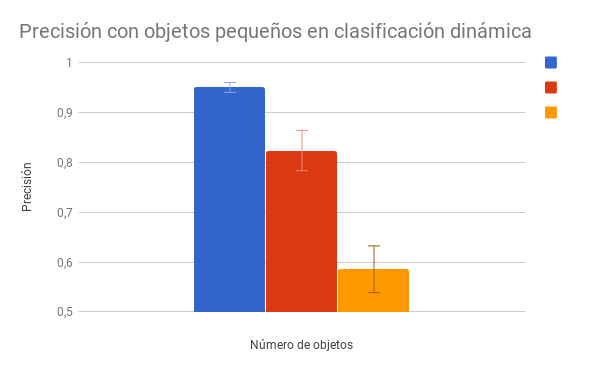
\includegraphics[scale=0.55]{imagenes/errbar_dp.png}
		\caption{Gráfica que muestra el número de objetos pequeños frente a la precisión en clasificación dinámica con cuña, representando la media con una columna y la desviación típica con una barra.}
	\end{figure}
	
	\noindent En la figura \ref{cd:dp} podemos ver que la utilización de objetos pequeños permite obtener mejores resultados en este entorno, ya que se consigue una eficiencia de casi 1 para 4 objetos, y para 6 y 7 no baja de 0.5. \\
	
\end{itemize} 

\noindent En definitiva, con los objetos pequeños se obtiene una mayor eficiencia en ambas clasificaciones, aunque esto se puede deber a las herramientas utilizadas, ya que no son las comunes que se utilizarían en una fábrica. Con las adecuadas se podrían obtener resultados preferentes a los mostrados en cuanto al peso o el área que ocupan en la mesa los objetos. \\